\documentclass{revtex4}
\usepackage{amsmath}
\usepackage{graphicx}
\usepackage{hyperref}
\begin{document}
\title{Lecture notes on probability and statistics relevant to experiments in PHYS 2501W}
\author{Prof. Andrew Puckett}
\affiliation{Dept. of Physics, University of Connecticut}
\date{\today}
\maketitle
\section{Definition of Probability Distribution, Mean, and Variance}
For a continuous random variable $x$, we define the probability density function or distribution $P(x)$ such that $\int_a^b P(x) dx$ is the probability that $x$ lies between $a$ and $b$. $P(x)$ is normalized so that its integral over all possible values of $x$ is one:
\begin{eqnarray}
  \int_{-\infty}^{\infty} P(x) dx = 1
\end{eqnarray}
We define the \emph{expectation value} of a function or operator $\mathcal{O}(x)$ as 
\begin{eqnarray}
  \left<\mathcal{O}(x) \right> &=& \int_{-\infty}^{\infty} \mathcal{O}(x) P(x) dx
\end{eqnarray}
We define the mean $\mu$ and the variance $\sigma^2$ of $x$ as 
\begin{eqnarray}
  \mu &=& \left<x\right> = \int_{-\infty}^\infty x P(x) dx \nonumber \\
  \sigma^2 &=& \left<(x-\mu)^2\right> = \int_{-\infty}^{\infty} (x - \mu)^2 P(x) dx \nonumber \\
  &=& \int_{-\infty}^{\infty} (x^2 - 2\mu x + \mu^2) P(x) dx = \left<x^2\right> - \left<x\right>^2
\end{eqnarray}
\section{Sampling statistics}
In experimental physics, we will often perform repeated measurements
of a quantity that is expected to have the same true value in each measurement, in order
to obtain an estimate of the uncertainty in the quantity, and to
reduce the uncertainty in that quantity by averaging several
independent measurements. In any individual measurement, the observed
value $x_{obs}$ will differ from the \emph{unknown} ``true'' value $x_t$
by an unknown amount $d_x = x_{obs} - x_t$. We can think of $x_{obs}$
as a random variable sampled from a probability distribution with mean
$\mu = x_t$ and standard deviation $\sigma$ characterizing the typical
error in a single measurement. Assuming
that our measurements are \emph{unbiased}, the theoretical mean of the
distribution of $x_{obs}$ is $\lim_{N \rightarrow \infty}
\left<\frac{1}{N} \sum_{i=1}^N x_i \right> = \mu = x_t$. In other words, we assume that we are
equally likely to err in either direction. Assume we have sampled the distribution of $x$ values by
performing $N$ measurements $x_i$ for $i=1,\ldots,N$. We define the \emph{sample mean} $\bar{x}$ and the \emph{sample variance} $s^2$ as 
\begin{eqnarray}
  \bar{x} &=& \frac{1}{N} \sum_{i=1}^{N} x_i \label{samplemean} \\
  s^2 &=& \frac{1}{N} \sum_{i=1}^{N} (x_i - \bar{x})^2 = \frac{1}{N} \sum_{i=1}^N x_i^2 -\frac{2}{N} \sum_{i=1}^{N} x_i \bar{x} + \frac{1}{N} \sum_{i=1}^N \bar{x}^2 \nonumber \\
  s^2 &=& \overline{x^2} - \bar{x}^2 \label{samplevariance},
\end{eqnarray}
where on the last line we have used the fact that
$\sum_{i=1}^N \bar{x}^2 =  N\bar{x}^2$ and
$\frac{-2}{N}\sum_{i=1}^N x_i \bar{x} = -2\bar{x}^2$. It follows from
the assumption of unbiased measurements that the expectation value of
the sample mean is simply the ``true'' value $x_t = \mu$. Second, let us
consider the variance of the sample mean. Since the expectation value
of the mean (the ``average of the average'') is $\mu$, the variance of
the sample mean is simply the average squared deviation of the mean of a sample of
size $N$ from the ``true'' value $\mu$:
\begin{eqnarray}
  \sigma_{\bar{x}}^2 &=& \left<(\bar{x} - \mu)^2 \right>
\end{eqnarray}
Let $d_i = x_i - \mu$ be the ``true error'' in a single measurement,
and let $D = \bar{x} - \mu$ be the ``true error'' in the sample mean. Then
$d_i - D = x_i - \bar{x}$ by definition.

The variance of the sample mean is evaluated by averaging $D^2$ over
the distribution of $x$:
\begin{eqnarray}
  \sigma^2_{\bar{x}} &=& \left<D^2\right> \nonumber \\
  &=& \left<\left(\frac{1}{N} \sum_{i=1}^N x_i - \mu\right)^2\right>
  \nonumber \\
  &=& \frac{1}{N^2}\left<\left(\sum_{i=1}^N x_i - N\mu \right)\left(\sum_{j=1}^N
      x_j - N\mu \right)\right> \nonumber \\
  &=& \frac{1}{N^2} \left<\left(\sum_{i=1}^N (x_i - \mu) \right)\left(\sum_{j=1}^N
      (x_j - \mu) \right) \right>\nonumber \\
  \sigma^2_{\bar{x}} &=& \frac{1}{N^2} \left<\sum_{i=1}^N d_i^2 +
    \sum_{i=1}^N \sum_{j \ne i}^N d_i d_j \right>  = \frac{\sigma^2}{N} \label{varianceofsamplemean},
\end{eqnarray}
where on the last line, we have replaced $(x_i - \mu)$ with $d_i$. Consider what happens when we take the expectation value in
Eq.~\eqref{varianceofsamplemean}. The expectation value of the ``true
error'' $d_i$ is zero by the assumption of unbiased
measurements. The second term inside the $\left<\ldots \right>$ in
Eq.~\eqref{varianceofsamplemean} vanishes because each of the $N$
measurements in each sample is assumed to be independent; i.e., the
error $d_i$ is uncorrelated with the error $d_j$ for $i \ne
j$. When we average this term over the distribution of a large number
of $N$-samplings, we get zero. Therefore, we are left with the term $\frac{1}{N^2}
\left<\sum_{i=1}^N d_i^2 \right>$. The expectation value
$\left<\sum_{i=1}^N d_i^2\right>$ just gives $N \left<d^2\right> = N
\sigma^2$, because each sample gives $N$ random $d^2$ values, and
the average of $d^2$ over the distribution is just $\sigma^2$, by
definition. We have thus arrived at the famous result that the
variance of the sample mean equals the variance of the parent distribution
divided by the number of measurements in the sample. Thus, if the
standard deviation $\sigma$ of the distribution of $x$ serves as a
measure of the error in a single measurement, then $\sigma_{\bar{x}}
= \sigma/\sqrt{N}$ serves as a measure of the error in the average
of $N$ independent measurements of the same quantity.

Let us consider next the relationship between the sample variance and
the distribution variance. The
expectation value of the sample variance is given by
\begin{eqnarray}
  \left<s^2 \right> &=& \frac{1}{N} \left<\sum_{i=1}^N (x_i -
    \bar{x})^2 \right> = \frac{1}{N} \left<\sum_{i=1}^N (d_i -D)^2
  \right> \nonumber \\
  &=& \frac{1}{N} \left<\sum_{i=1}^N \left( d_i^2 + D^2 - 2d_i D
    \right)\right> \nonumber \\
  &=& \sigma^2 + \frac{\sigma^2}{N} - \frac{2}{N} \left<\sum_{i=1}^N
    (x_i-\mu)(\bar{x}-\mu)\right> = \sigma^2 + \frac{\sigma^2}{N} -
  \frac{2}{N} \left<N (\bar{x}-\mu)^2 \right> \nonumber \\
  &=& \sigma^2 + \frac{\sigma^2}{N} - \frac{2}{N}\left<N D^2 \right> =
  \sigma^2 - \frac{\sigma^2}{N} = \sigma^2 \frac{N-1}{N} 
\end{eqnarray}
We therefore see that the sample variance is a \emph{biased} estimator for the
variance of the distribution, and tends to underestimate the variance
at small values of $N$. As $N$ becomes large, however, the factor
$(N-1)/N$ multiplying $\sigma^2$ tends toward one. Moreover, we see
that $s^2 \frac{N}{N-1} = \frac{1}{N-1}\sum_{i=1}^N (x_i - \bar{x})^2$
is an \emph{unbiased} estimator for $\sigma^2$.
\section{Special Probability Distributions: Binomial, Poisson and
  Gaussian}
\subsection{Binomial}
The binomial distribution describes the probability distribution of outcomes of
binary (success/failure) experiments. Specifically, the probability
$P(k)$ of observing $k$ ``successes'' in $N$ independent trials when the
probability of success is $p$ is given by:
\begin{eqnarray}
  P(k) &=& \frac{N!}{k!\left(N-k\right)!} p^k (1-p)^{N-k} \label{binomialdist}
\end{eqnarray}
The various factors appearing in Eq.~\eqref{binomialdist} are
intuitively simple to understand. The factor $p^k$ represents the product of the
individual probabilities of each of the $k$ successes. The factor
$(1-p)^{N-k}$ represents the product of the individual probabilities
for each of the $N-k$ failures. However, we don't care about the order
in which the successes and failures occur, so we have to multiply this
probability by the number of possible ways of choosing $k$ successes
from $N$ trials. It is a well-known fact that the number of possible
orderings of $N$ trials, regardless of success or failure, is
$N!$. Let $M$ be the number of possible orderings of $k$ successes
drawn from among $N$ trials. There are $N$ ways to choose the first
(successful) trial. For each possible choice of the first trial, there
are $N-1$ ways to choose the second trial, and so on all the way up to $N - k + 1$ ways to choose
the $k^{th}$ trial: 
\begin{eqnarray}
  M &=& N (N-1) (N-2) \ldots (N-k + 1) = N (N-1) (N-2) \ldots (N-k +
  1) \times \frac{(N-k)!}{(N-k)!} = \frac{N!}{(N-k)!}
\end{eqnarray}
Recalling that we don't care about the ordering of the $k$ successes,
the number of ways of choosing $k$ successes from $N$ trials is simply
given by $M/k! = \frac{N!}{k!(N-k)!}$.

\begin{figure}[h]
  \begin{center}
    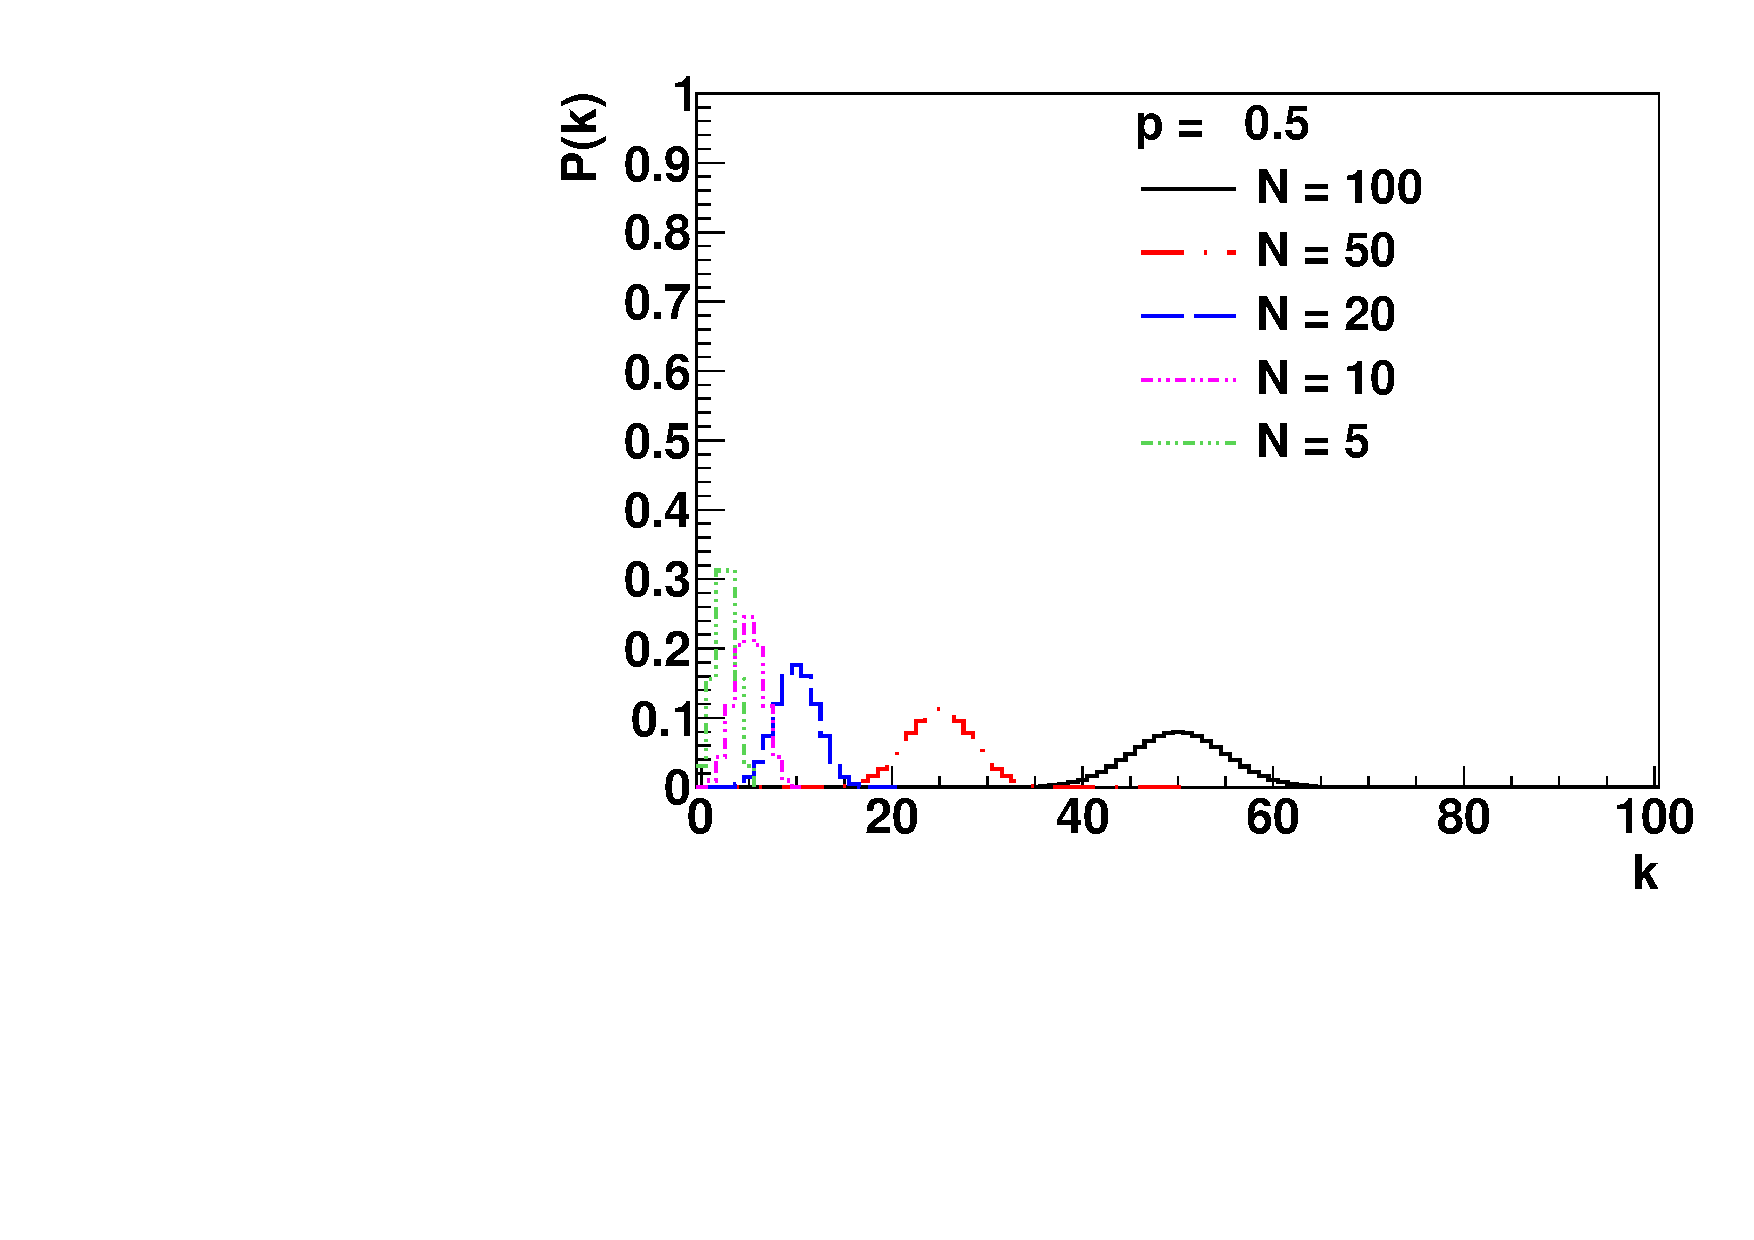
\includegraphics[width=0.48\textwidth]{Binomial_vs_N_p50.pdf}
    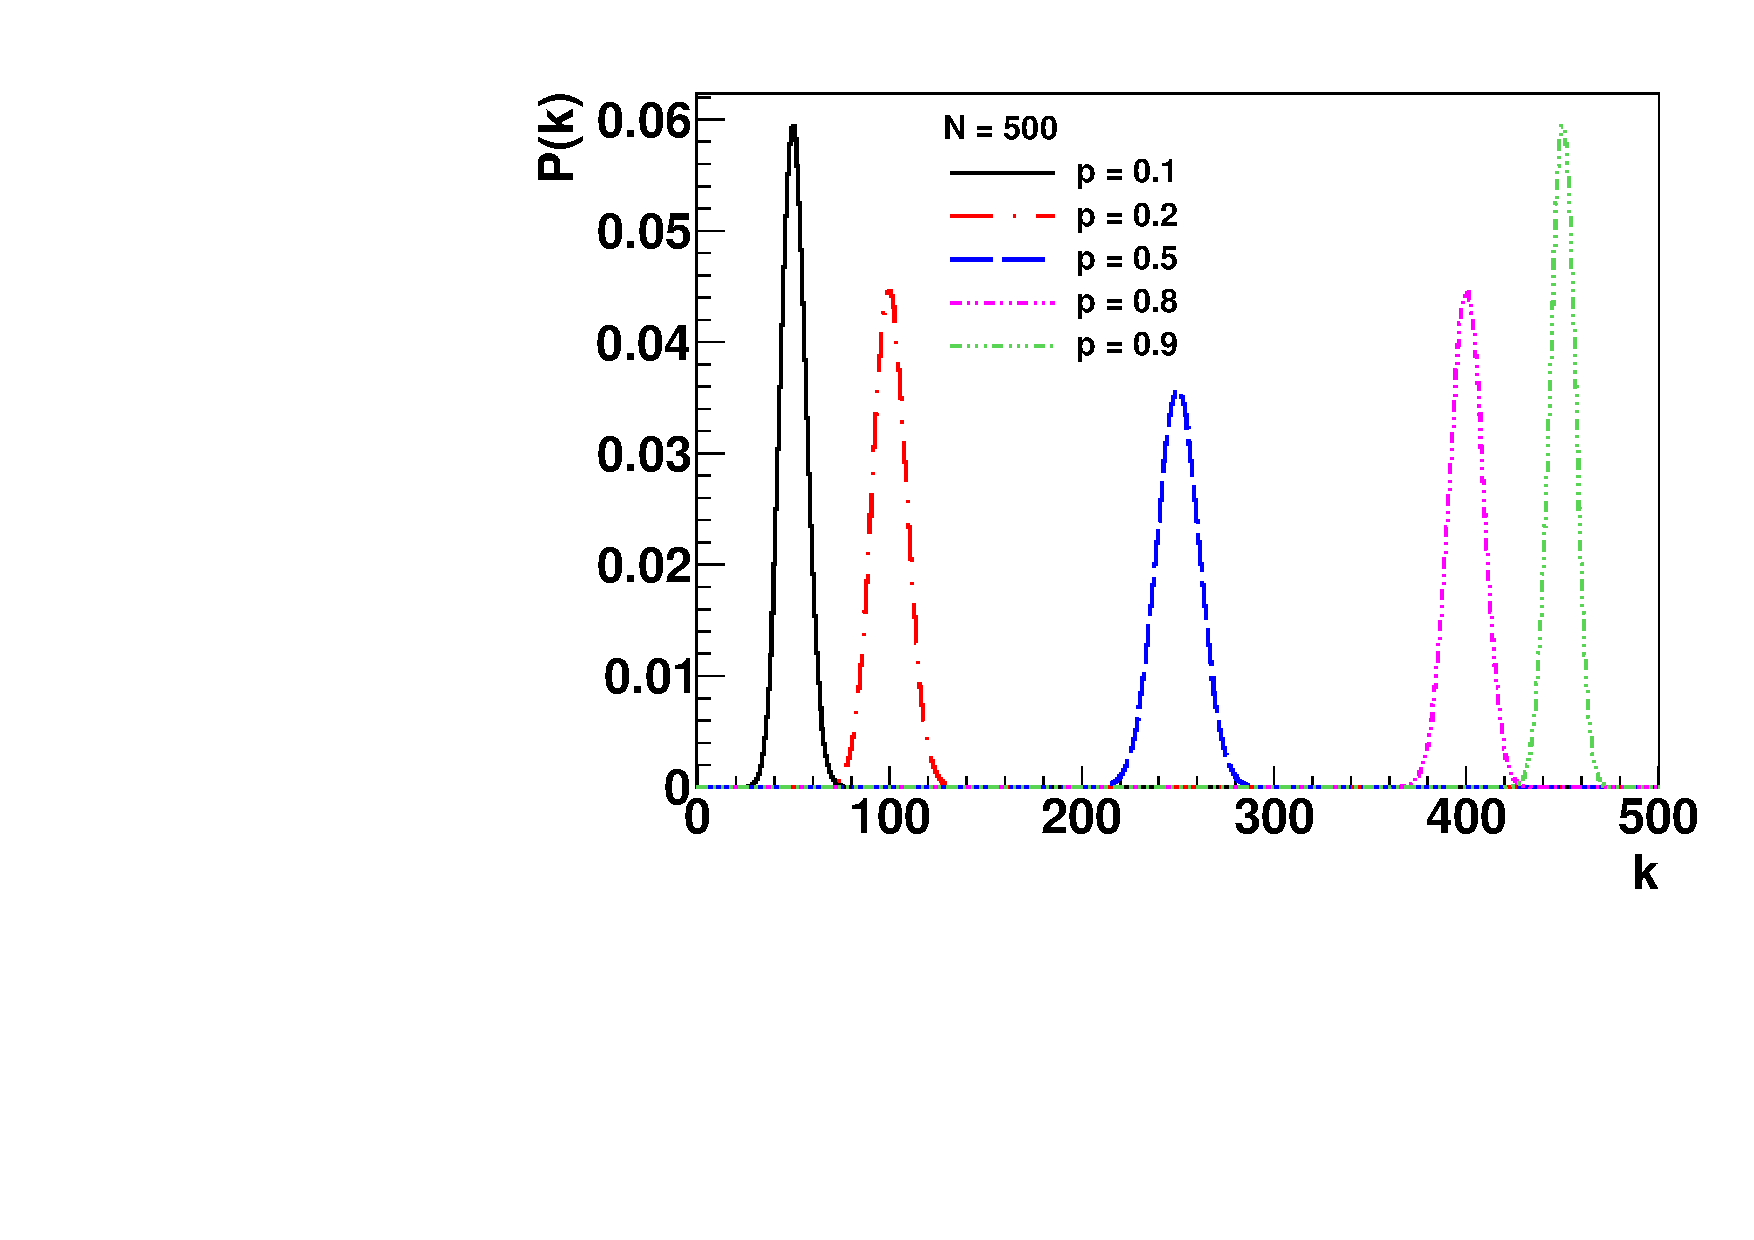
\includegraphics[width=0.48\textwidth]{Binomial_vs_p_N500.pdf}
  \end{center}
  \caption{\label{fig:binomial} Left: Binomial distribution at
    different values of $N$ for a fixed $p=0.5$. Right: Binomial
    distribution at different values of $p$ for a fixed $N = 500$.}
\end{figure}
Figure \ref{fig:binomial} shows the behavior of the binomial
distribution $P(k)$ as a function of $N$ for fixed $p$, and as a
function of $p$ for fixed $N$. We see that the average and most
probable value of $k$ is $Np$, and that the fractional deviations of
$k$ from $Np$ decrease as $N$ increases. A more quantitative statement
of this observation will be made below. The binomial distribution can be shown to be normalized (i.e., that
$\sum_{k=0}^N P(k) = 1$) by simply recognizing the fact that this sum
is equivalent to the binomial expansion of $((1-p)+p)^N = 1$. Indeed,
this is where the name ``Binomial'' distribution comes from. The mean of the binomial distribution is given by $\left<k\right> =
Np$. This can be shown by carrying out the sum of $k P(k)$ over all
$k$ from 0 to N:
\begin{eqnarray}
  \left<k\right> &=& \sum_{k=0}^N k P(k) \nonumber \\
  &=& \sum_{k=0}^N k \frac{N!}{k! (N-k)!} p^k (1-p)^{N-k} \nonumber \\
  &=& \frac{p}{1-p} \sum_{k=1}^N \frac{N!(N-k+1)}{(k-1)! (N-k+1)!} p^{k-1}(1-p)^{N-k+1} \nonumber \\
  &=& \frac{p}{1-p} \sum_{k=0}^{N-1} (N-k) P(k) = \frac{p}{1-p}
  \left[N\sum_{k=0}^{N-1} P(k) - \sum_{k=0}^{N-1} k P(k)\right]
  \nonumber \\
  \left<k\right> &=& \frac{p}{1-p}\left[N(1-p^N) - \left<k\right> + N p^N \right] =
  \frac{p}{1-p}(N-\left<k\right>) \nonumber \\
  \left(1-p+p\right)\left<k\right> = \left<k\right> &=& Np \label{binomial_mean}
\end{eqnarray}
The variance of the binomial distribution is given by $\sigma_k^2 =
Np(1-p)$, as is shown by computing the sum of $(k-Np)^2 P(k)$ over all $k$:
\begin{eqnarray}
  \sigma_k^2 + (Np)^2 &=& \sum_{k=0}^N k^2 P(k) \nonumber \\
  &=& \sum_{k=1}^N k \frac{N!}{(k-1)! (N-k)!} p^k(1-p)^{N-k} \nonumber
  \\
  &=& \frac{p}{1-p}\sum_{k=1}^N k\frac{N! (N-k+1)}{(k-1)!(N-k+1)!}
  p^{k-1}(1-p)^{N-k+1} \nonumber \\
  &=& \frac{p}{1-p} \sum_{k=1}^N k (N-k+1) P(k-1) =
  \frac{p}{1-p}\sum_{k=0}^{N-1} (k+1)(N-k) P(k) \nonumber \\
  &=& \frac{p}{1-p} \left[N \sum_{k=0}^{N-1} kP(k) + N
    \sum_{k=0}^{N-1} P(k) - \sum_{k=0}^{N-1} k^2 P(k) -
    \sum_{k=0}^{N-1} k P(k) \right] \nonumber \\
  &=& \frac{p}{1-p} \left[N( Np - Np^N) + N - Np^N - \left<k^2\right>
    + N^2 p^N - Np + Np^N \right] \nonumber \\
  &=& \frac{p}{1-p}\left[N^2 p  + N - \left<k^2\right> - Np  \right] =
  \frac{p}{1-p}\left[N(Np + 1 - p) - \left<k^2\right> \right]
  \nonumber \\
  \left<k^2\right> &=& Np(Np + 1 - p) = (Np)^2 + Np(1-p) \nonumber \\
  \Rightarrow \sigma_k^2 &=& Np(1-p)
\end{eqnarray}
The standard deviation $\sigma_k$ of $k$ is then given by 
\begin{eqnarray}
  \frac{\sigma_k}{\left<k\right>} &=& \frac{\sqrt{Np(1-p)}}{Np} = \sqrt{\frac{1-p}{Np}}
\end{eqnarray} 
Therefore we see that at fixed $p$, the fractional spread of $k$ about
the mean $Np$ decreases as $1/\sqrt{N}$ as $N$ becomes large.
\subsection{Poisson}
The Poisson distribution emerges from consideration of the Binomial
distribution in the limit as $N \rightarrow \infty$ and $p \rightarrow
0$ while the product $Np = \lambda$ remains finite, approaching a
constant value $\lambda$. A good example of a physical system governed
by Poisson statistics is a sample of low-level, long-lived radioactive
material such as $^{238}$U. The lifetime of $^{238}$U is long enough
that the number of nuclei present does not change by a measurable
amount over any reasonable time interval we can observe in the
lab. Therefore, the counting rate $R = dN/dt$, the number of decays
observed per unit time, is constant to a very good approximation.  When we observe the activity level of such
a source using a Geiger counter to count the number of decays in a
time interval $T$, the probability of any individual nucleus decaying
is very small (close to zero), whereas the number of unstable nuclei
in the sample is large, such that the expected average number of counts
$\lambda = RT$ is finite. Consider Eq.~\eqref{binomialdist} in the
limit of large $N$ and small $p$, with $Np = \lambda = $ constant. 
\begin{eqnarray}
  \lim_{N \rightarrow \infty, Np \rightarrow \lambda}
  \frac{N!}{k!(N-k)!} p^k (1-p)^{N-k} &=& \lim_{N \rightarrow
    \infty,Np \rightarrow \lambda} \frac{N(N-1)(N-2)\ldots
    (N-k+1)(N-k)!}{k!(N-k)!}p^k(1-p)^{N-k} \nonumber \\
  &=& \frac{(Np)^k}{k!} \lim_{N\rightarrow \infty, Np \rightarrow \lambda} (1-p)^{N-k} =
  \frac{\lambda^k}{k!} \lim_{N\rightarrow \infty, Np\rightarrow \lambda} (1-p)^N \nonumber \\
 \ln \left((1-p)^N\right) = N \ln (1-p) &\xrightarrow[p \rightarrow 0]{}& -Np = -\lambda \nonumber \\
 \Rightarrow \lim_{N\rightarrow \infty,Np\rightarrow \lambda} P(k) &=&
 \frac{\lambda^k e^{-\lambda}}{k!} \label{PoissonDist}
\end{eqnarray}
The discrete probability distribution represented by
Eq.~\eqref{PoissonDist} is known as the Poisson distribution. It is
easy to show that the Poisson distribution is normalized by noting
that $\sum_{n=0}^\infty P(n) = \sum_{n=0}^\infty \frac{\lambda^n
  e^{-\lambda}}{n!} = e^{-\lambda} \sum_{n=0}^\infty
\frac{\lambda^n}{n!} = e^{-\lambda}e^\lambda = 1$. The mean
and variance of the Poisson distribution can be computed as follows:
\begin{eqnarray}
  \left<n\right> &=& \sum_{n=0}^\infty n P(n) = \sum_{n=0}^\infty n
  \frac{\lambda^n e^{-\lambda}}{n!}  \nonumber \\
  &=& \sum_{n=1}^\infty \frac{\lambda^n e^{-\lambda}}{(n-1)!} =
  \lambda \sum_{m=0}^\infty \frac{\lambda^m e^{-\lambda}}{m!} = \lambda
\end{eqnarray}
The result for the mean is obvious since $\lambda$ was defined from
the beginning as the average value of $n$. The variance $\sigma_n^2 =
\left<\left(n-\left<n\right>\right)^2\right>$ is given by:
\begin{eqnarray}
  \sigma_n^2 + \lambda^2 &=& \sum_{n=0}^\infty n^2 P(n)  \nonumber \\
  &=& \sum_{n=1}^\infty n \frac{\lambda^n e^{-\lambda}}{(n-1)!}
  \nonumber \\
  &=& \lambda \sum_{m=0}^\infty (m+1) \frac{\lambda^m
    e^{-\lambda}}{m!} \nonumber \\
  &=& \lambda (\lambda + 1) \nonumber \\
  \Rightarrow \sigma_n^2 &=& \lambda(\lambda+1) - \lambda^2 = \lambda
\end{eqnarray}
Thus we have arrived at the well-known result that both the mean and the
variance of the Poisson distribution are equal to $\lambda$, and
therefore the standard deviation of the Poisson distribution divided
by the mean value is $\sigma_n/\left<n\right> = 1/\sqrt{\lambda}$. Now
let us consider the Poisson distribution in the limit of large
$\lambda$. We start by taking the logarithm of $P(n)$:
\begin{eqnarray}
  \ln{P(n)} &=& n \ln \lambda - \lambda - \ln n! \label{logPn}
\end{eqnarray}
Let $x = (n - \lambda)/\lambda$, so that $n = \lambda(1 + x)$. In the
limit of large $\lambda$, the standard deviation of $n$ vanishes as
$1/\sqrt{\lambda}$, so that in this limit, $x$ can be considered
small. Replacing $n$ with $\lambda(1+x)$, equation~\eqref{logPn} becomes:
\begin{eqnarray}
  \ln P(n) &=& \lambda(1+x) \ln \lambda - \lambda - \ln\left(
    (\lambda(1+x))! \right)
\end{eqnarray}
Consider the last term with the factorial on the right-hand-side. The
factorial of $n$ can be written in integral form as 
\begin{eqnarray}
  n! &=& \int_0^\infty x^n e^{-x} dx \label{nfactintegral}
\end{eqnarray}
To see why this is the case, carry out the integral on the
right-hand-side using integration by parts. Let $u = x^n$ and $dv =
e^{-x} dx$. Then $v = -e^{-x}$ and $du = nx^{n-1}$, and the integral can
be rewritten as: 
\begin{eqnarray}
  n! &=& \left. -x^n e^{-x}\right|_0^\infty + n \int_0^\infty x^{n-1}
  e^{-x} dx
\end{eqnarray}
The first term vanishes because it gives zero at $x=0$ and $x=\infty$, while the second term gives $n(n-1)! = n!$
(assuming validity of Eq.~\eqref{nfactintegral}). We can prove that
Eq.~\eqref{nfactintegral} is valid for integer $n$ by carrying out
integration by parts all the way down to $n=1$:
\begin{eqnarray}
  \int_0^\infty x^n e^{-x} &=& n \int_0^\infty x^{n-1}e^{-x} dx =
  n(n-1) \int_0^\infty x^{n-2}e^{-x}dx \nonumber \\
  &=& n(n-1)(n-2)\ldots(2)(1) \int_0^\infty e^{-x} dx = n!
\end{eqnarray}
Using the integral form of $n!$, we can derive an approximation known
as Stirling's approximation for $\ln n!$ in the limit of large
$n$. Consider the logarithm of the integrand of
Eq.~\eqref{nfactintegral}:
\begin{eqnarray}
  \ln \left(x^n e^{-x} \right) &=& n \ln x - x
\end{eqnarray}
In the limit of large $n$, the integrand is strongly peaked around $x
= n$ (this is also true of the Poisson distribution). Let $x = n(1+
\delta)$, where $\delta$ will be taken to be small later on.
\begin{eqnarray}
  \ln \left(x^n e^{-x} \right) &=& n \ln (n(1+\delta)) - n(1+\delta)
  \nonumber \\
  &=& n \ln n + n \ln (1+\delta) - n(1+\delta) \nonumber \\
  &\approx& n \ln n + n\left(\delta - \frac{\delta^2}{2} +
    \mathcal{O}\left(\delta^3\right)\right) -n(1+\delta) \nonumber \\
  \ln \left(x^n e^{-x} \right) &\approx & n \ln n - n - n
  \frac{\delta^2}{2} \label{eq23}
\end{eqnarray}
Exponentiating both sides of Eq.~\eqref{eq23}, we find:
\begin{eqnarray}
  x^n e^{-x} &\approx& n^ne^{-n} e^{-n\frac{\delta^2}{2}}
\end{eqnarray} 
so that the integral equation for $n!$ can be rewritten as
\begin{eqnarray}
  n! &\approx & n^ne^{-n} \int_{-1}^{\infty}
  \frac{e^{-n\frac{\delta^2}{2}}}{n} d\delta = n^n e^{-n}
  \int_{-n}^\infty e^{-\frac{y^2}{2n}} dy \approx n^n e^{-n}
  \int_{-\infty}^{\infty} e^{-\frac{y^2}{2n}} dy, \label{nfactapprox}
\end{eqnarray}
where in the last step, we have extended the lower limit of the
integral to $-\infty$, reflecting the large-$n$ approximation. The
integral of $e^{-\frac{y^2}{2n}} dy$ can be carried out by squaring
the integral and then switching to polar coordinates:
\begin{eqnarray}
  \left( \int_{-\infty}^\infty e^{-\frac{y^2}{2n}} dy\right)^2 &=& \left(
    \int_{-\infty}^\infty e^{-\frac{y^2}{2n}} dy \right)\left( \int_{-\infty}^\infty
    e^{-\frac{x^2}{2n}} dx \right) \nonumber \\
  &=& \int_0^{2\pi} \left[\int_0^\infty r e^{-\frac{r^2}{2n}} dr
  \right] d\phi \nonumber \\
  &=& 2\pi n \int_0^\infty e^{-u} du = 2\pi n \nonumber \\
  \int_{-\infty}^{\infty} e^{-\frac{y^2}{2n}} dy &=& \sqrt{2\pi n}
\end{eqnarray} 
Substituting this expression back into the
expression~\eqref{nfactapprox} for $n!$, we finally find
\begin{eqnarray}
  n! &\approx& n^n e^{-n} \sqrt{2\pi n} \\
  \ln (n!) &\approx & n \ln n - n + \frac{1}{2} \ln (2\pi n) \label{Stirling}
\end{eqnarray}
Equation~\eqref{Stirling} is known as Stirling's
approximation. Sometimes only the first two terms are retained, as the
third term is small compared to the first two in the large $n$
limit. To analyze the limiting behavior of the Poisson distribution,
however, we keep this term. Substituting Stirling's approximation for
$\ln n!$ back into the expression~\eqref{logPn} for $\ln(P(n))$, and
letting $n = \lambda(1+x)$, we
find 
\begin{eqnarray}
  \ln P(n) &=& n \ln \lambda - \lambda - \left[n \ln n - n +
    \frac{1}{2}\ln(2\pi n) \right] \nonumber \\
  &=& \lambda(1+x) \ln \lambda - \lambda -
  \left[\lambda(1+x)\ln(\lambda(1+x)) - \lambda(1+x) + \frac{1}{2} \ln(2\pi\lambda(1+x))\right],
\end{eqnarray}
which simplifies to 
\begin{eqnarray}
  \ln P(n) &\approx& \lambda(1+x)\ln \lambda - \lambda - \lambda(1+x)(\ln \lambda +
  \ln(1+x)) + \lambda(1+x) - \frac{1}{2} \ln(2\pi \lambda(1+x))
  \nonumber \\
  &=& -\lambda(1+x)\ln(1+x) + \lambda x - \frac{1}{2} \ln (2\pi
  \lambda(1+x)) \nonumber \\
  &\approx& -\lambda(1+x)\left(x - \frac{x^2}{2} +
    \mathcal{O}(x^3)\right) + \lambda x - \frac{1}{2} \ln (2\pi
  \lambda(1+x)) \nonumber \\
  &\approx& -\lambda \left(x + x^2 - \frac{x^2}{2} +
    \mathcal{O}(x^3)\right) + \lambda x - \frac{1}{2} \ln(2\pi
  \lambda(1+x)) \nonumber \\
  &\approx & -\lambda \frac{x^2}{2} -\frac{1}{2} \ln(2\pi \lambda),
\end{eqnarray}
where on the last line, we have replaced $1+x \rightarrow 1$ in the
argument of the logarithm in the second term. This is justified
because the $x$-dependence of the second term vanishes in the
large-$\lambda$ limit.
  
Exponentiating this expression leads to a large-$\lambda$
approximation for $P(n)$:
\begin{eqnarray}
  P\left(x = \frac{n-\lambda}{\lambda}\right) &=& \frac{e^{-\frac{\lambda
        x^2}{2}}}{\sqrt{2\pi \lambda}}.
\end{eqnarray}
If we define $y = \lambda x = n - \lambda$, then the large-$\lambda$ limit
of $P(y)$ is 
\begin{eqnarray}
  P(y = n - \lambda) &=& \frac{e^{-\frac{y^2}{2\lambda}}}{\sqrt{2\pi \lambda}}
\end{eqnarray}
Thus, in the limit of large $\lambda$, the Poisson distribution
approaches a Gaussian or normal distribution with mean $\lambda$
and standard deviation $\sqrt{\lambda}$. This brings us to the
discussion of one of the most important distributions in statistics
and experimental physics, the Gaussian or normal distribution.
\subsection{Gaussian (Normal) Distribution}
The Gaussian distribution with mean $\mu$ and standard deviation
$\sigma$ for a continuous random variable $x$ is defined as
\begin{eqnarray}
  P(x) &=& \frac{1}{\sqrt{2\pi \sigma^2}}e^{-\frac{(x-\mu)^2}{2\sigma^2}}
\end{eqnarray}
It is normalized so that its integral over all $x$ gives one:
\begin{eqnarray}
  \int_{-\infty}^\infty P(x) dx &=& \frac{1}{\sqrt{2\pi \sigma^2}}
  \int_{-\infty}^\infty e^{-\frac{(x-\mu)^2}{2\sigma^2}} dx =
  \frac{\sqrt{2\pi \sigma^2}}{\sqrt{2\pi\sigma^2}} = 1
\end{eqnarray}
It can be shown that the expectation value for the normal distribution
is $\mu$ as follows:
\begin{eqnarray}
  \left<x\right> &=& \frac{1}{\sqrt{2\pi\sigma^2}}
  \int_{-\infty}^{\infty} x e^{-\frac{(x-\mu)^2}{2\sigma^2}} dx
\end{eqnarray}
Let $y = \frac{x-\mu}{\sigma}$. Then $dy = dx/\sigma$ and the
exponential becomes $e^{-\frac{y^2}{2}}$. $x dx$ becomes $(\sigma y +
\mu) \sigma dy$, so that the integral becomes
\begin{eqnarray}
  \left<x\right> &=& \frac{1}{\sqrt{2\pi \sigma^2}}
  \int_{-\infty}^\infty \left(\sigma^2 y + \sigma \mu\right)
    e^{-\frac{y^2}{2}} dy \label{Gaussmean} \\
    &=& \frac{1}{\sqrt{2\pi \sigma^2}} \mu \sigma
    \int_{-\infty}^\infty e^{-\frac{y^2}{2}} dy = \mu
\end{eqnarray}
The first term in Eq.~\eqref{Gaussmean} vanishes because
$ye^{-\frac{y^2}{2}}$ is an odd function, integrated over the entire
real axis. The integral of the second term just gives $\sigma \mu
\sqrt{2\pi}$, which cancels the normalization constant in the
denominator and leaves us with $\mu$. We can similarly show that the
variance of the normal distribution is $\sigma^2$:
\begin{eqnarray}
  \left<(x-\mu)^2\right> &=& \frac{1}{\sqrt{2\pi \sigma^2}}
  \int_{-\infty}^\infty (x-\mu)^2 e^{-\frac{(x-\mu)^2}{2\sigma^2}} dx
\end{eqnarray}
Again, we make the simplifying substitution $y = \frac{x-\mu}{\sigma}$:
\begin{eqnarray}
  \left<(x-\mu)^2\right> &=& \frac{\sigma^2}{\sqrt{2\pi}}
  \int_{-\infty}^\infty y^2 e^{-\frac{y^2}{2}} dy
\end{eqnarray}
The integral can be carried out using integration by parts. Let $u =
y$ and $dv = ye^{-\frac{y^2}{2}} dy$. Then $uv = -ye^{-\frac{y^2}{2}}$
and $-v du =e^{-\frac{y^2}{2}} dy$:
\begin{eqnarray}
  \left<(x-\mu)^2\right> &=& \frac{\sigma^2}{\sqrt{2\pi}}
  \left[\left.-ye^{-\frac{y^2}{2}}\right|_{-\infty}^{\infty} +
    \sqrt{2\pi} \right] = \sigma^2
\end{eqnarray}
\begin{figure}[h]
  \begin{center}
    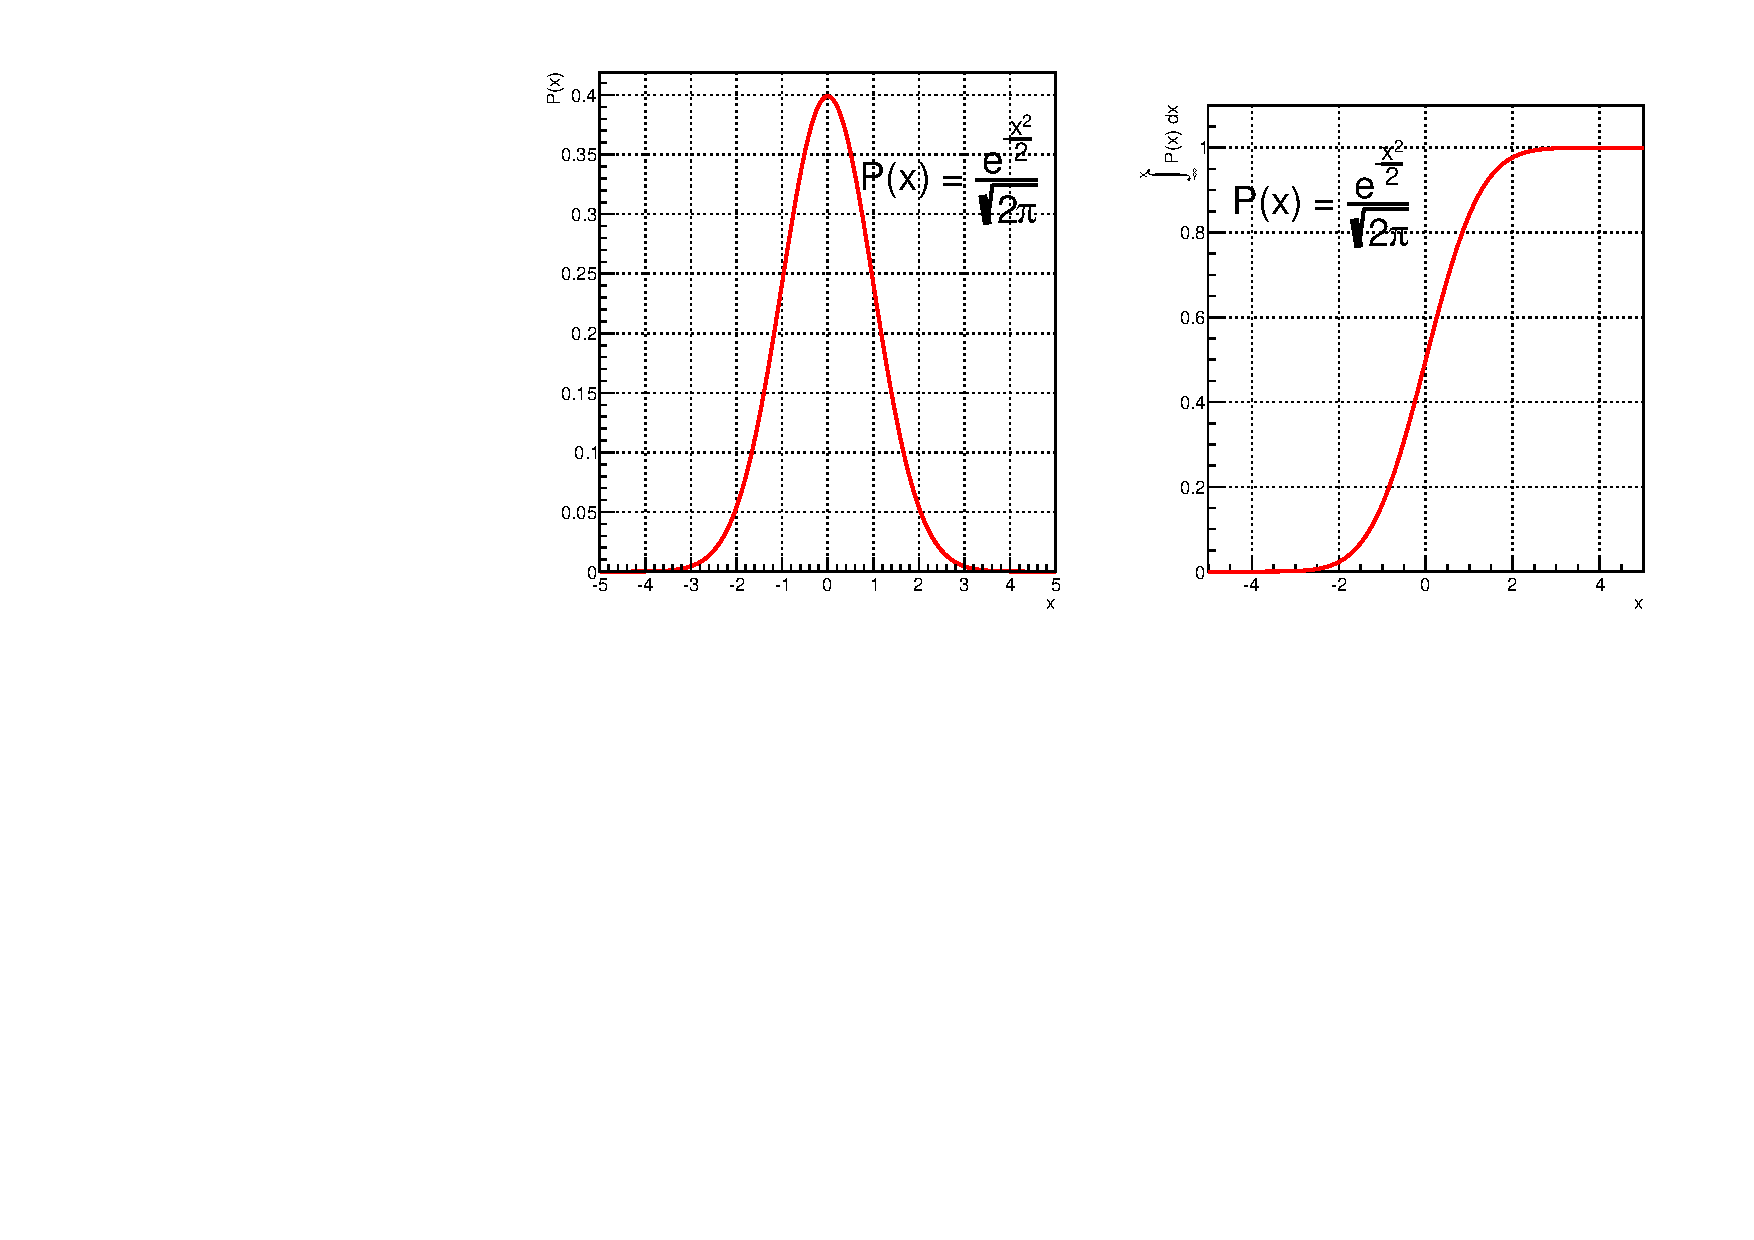
\includegraphics[width=.98\textwidth]{Gaussian.pdf}
  \end{center}
  \caption{\label{fig:Gauss} Normal distribution with mean $\mu = 0$ and
    standard deviation $\sigma = 1$. Left: Gaussian distribution $P(x)$. Right: The
    cumulative distribution function $C(x) = \int_{-\infty}^x P(x') dx'$
    representing the cumulative probability that a randomly sampled
    observation $x'$ will give a result $x' \le x$.}
\end{figure}
Figure~\ref{fig:Gauss} shows the behavior of the Gaussian distribution
$P(x)$ with mean $\mu = 0$ and standard deviation $\sigma = 1$, as
well as its cumulative distribution function. According to the Central Limit
Theorem presented in the next section, if $(x_i; i=1,\ldots,N)$ are
independent random variables sampled from \emph{any} distribution with finite mean $\mu$ and finite
variance $\sigma^2$, then in the limit as $N \rightarrow \infty$, the
variable $\bar{x} = \frac{1}{N} \sum_{i=1}^N x_i$ is normally
distributed with mean $\mu$ and variance $\sigma_{\bar{x}}^2 =
\sigma^2/N$. Therefore, if we perform a large number of repeated
measurements of the same quantity that is subject to random
measurement errors characterized by a standard deviation $\sigma$, the
Central Limit Theorem helps us to relate $\sigma$ to a 

\section{The Central Limit Theorem}
\section{The $\chi^2$ distribution, the Least-Squares method, and the
  meaning of $\chi^2$ as a test of goodness-of-fit}

\end{document}
